\section{Digitale Datenübertragung über AWGN-Kanal}
\begin{center}
	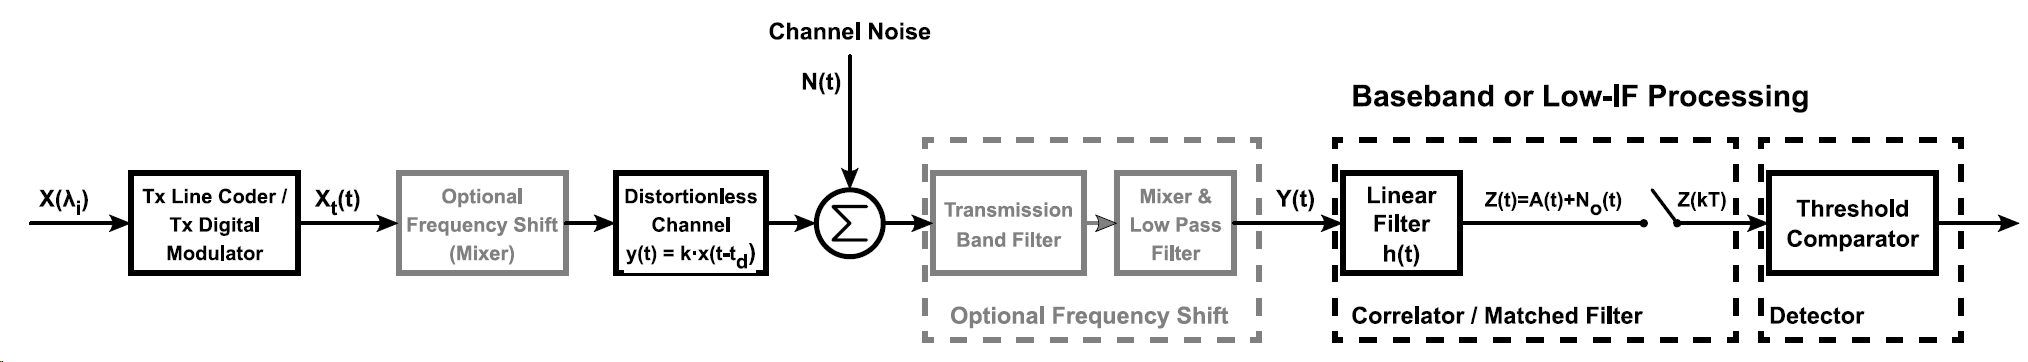
\includegraphics[width=\columnwidth]{Images/awgn_digital}
\end{center}

\subsection{Maximum A-Posteriori Detektor - MAP}
\script{191} Bei \textit{ungleich häufigen} Mark und Space, wird das MAP-Kriterium angewendet. Die \textbf{Bitfehlerwahrscheinlichkeit} $p_e$ beim Empfänger:
\[
p_e = Q\left(\frac{|a_1 - \lambda_0|}{\sigma_{n_o}}\right)\cdot P(S_1) + Q\left(\frac{|a_2 - \lambda_0|}{\sigma_{n_o}}\right)\cdot P(S_2)
\]
\begin{center}
	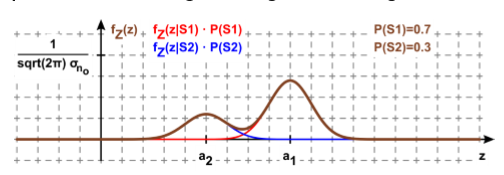
\includegraphics[width=0.8\columnwidth]{Images/map}
\end{center}
Die Entscheidungsschwelle $\lambda_0$ entspricht dabei $\lambda_0 = \frac{a_1 + a_2}{2} + \frac{\sigma_{n_o}^2}{a_1 - a_2}\cdot\ln\left(\frac{P(S_2)}{P(S_1)}\right)$


\subsection{Maximum Likelihood Detektor - ML}
\script{194} Wenn $P(S_1) = P(S_2)$, bzw. Mark und Space \textit{gleich häufig} vorkommen, ist die \textbf{Bitfehlerwahrscheinlichkeit} $p_e$ beim Empfänger.
\[
p_e = Q\left(\frac{|a_1 - a_2|}{2\sigma_{n_o}}\right) \geq Q\left(\sqrt{\frac{E_d}{2\eta}}\right)
\]
Die Entscheidungsschwelle $\lambda_0$ entspricht dabei $\lambda_0 = \frac{a_1 + a_2}{2}$
\begin{center}
	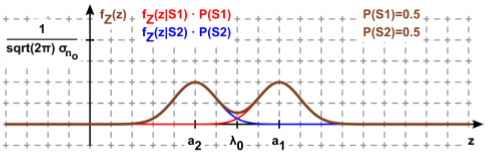
\includegraphics[width=0.8\columnwidth]{Images/ml}
\end{center}
\noindent\textbf{Beispiel} Bipolares NRZ-Signal mit Zero-Order Hold Signal während Bitzeit $T$. $s_1$ und $s_2$ sind gleich häufig:\\
\begin{align*}
	\text{Mark: } s_1(t) = A &\qquad \text{Space: } s_2(t) = -A\\
	P(s_1) = P(s_2) &= \frac{1}{2}
\end{align*}
AWGN-Rauschen hat eine konstante spektrale Leistungsdichte $S_{NN}(\omega) = \frac{\eta}{2}$. Das Differenzsignal über Symbolzeit $T$ entspricht $s(t) = s_1(t) - s_2(t) = 2\cdot A$. Die Differenzenergie entspricht $E_d = 4\cdot A^2\cdot T$. Damit lässt sich die Bitfehlerwahrscheinlichkeit berechnen:
\begin{align*}
	p_e \ge Q\left(\sqrt{\frac{E_d}{2\eta}}\right) = Q\left(\sqrt{\frac{4\cdot A^2 \cdot T}{2\eta}}\right)
\end{align*}
Die mittlere Leistung bei je $50\%$ Mark und Space $\overline{P} = \frac{1}{2}A^2 + \frac{1}{2}A^2 = A^2$.
\[
p_e = Q\left(\sqrt{\frac{2\cdot \overline{P} \cdot T}{\eta}}\right)
\]

Siehe \script{262} für Q-Funktion Tabelle.

\subsection{Optimaler Matched Filter}\script{195}
Dieses Filter ist an die Signalformen $s_{1,2}$ angepasst, sodass der Unterschied zwischen Mark und Space zum Abtastzeitpunkt $t =k\cdot T$ maximiert und gleichzeitig den Rauschanteil minimiert. Dies führt zur Minimalen Bitfehlerrate $p_e$!

Grafisch kann die Impulsantwrot $h(t)$ des Matched Filters sehr einfach konstruiert werden:
\begin{itemize}[nosep]
	\item Spiegeln des Differenzsignals $s(t) = s_1(t) - s_2(t)$ an der Y-Achse
	\item Anschliessend $s(t)$ verzögern (nach rechts schieben) des gespiegelten Signals um $T$
\end{itemize}